


\section{Descripción General del Desarrollo del Protocolo}
El protocolo criptográfico para evitar duplicados almacenados en la nube, es un proyecto que involucra la tecnología de software para ofrecer un funcionamiento eficiente y útil para las necesidades de los usuarios que se encuentran inmersos en el cómputo nube. 
Nuestro protocolo, se compone a su vez de diferentes módulos. Cada uno de ellos busca satisfacer: \\ 

\begin{itemize}

\item La seguridad de los archivos de los usuarios en la nube
\item Almacenamiento seguro en la sube
\item Conexión de diversos usuarios 
\item Ahorro en el consumo de espacio ofrecido en la nube 
\item Fácil acceso al almacenamiento de los archivos de los usuarios 

\end{itemize} 

Para lograrlo, el protocolo criptográfico se compone de diversos módulos que a su vez integran diferentes aplicaciones criptográficas. Dichos módulos serán detallados en las próximas secciones. 

\section{Servidor de Llaves}
El módulo Servidor de llaves tiene una función muy importante dentro del funcionamiento del protocolo criptográfico, ya que sin dicho servidor los usuarios no podrían conectarse para poder utilizar el servicio de almacenamiento seguro. 
En éste módulo participan: 
\begin{itemize}
	\item El factor de ocultamiento (Proporcionado por el cliente)
	\item La clave privada del servidor \textit{d} , generada mediante el algoritmo RSA. 
	\end{itemize}

El desarrollo de éste módulo, fué realizado mediante el lenguaje de programación Python en su versión 2.7. \\
Las librerías utilizadas para llevar a cabo la implementación de éste móludo son: 

			\begin{figure}[H]
			\centering
			\includegraphics[width=9cm, height=2.3cm]{./images/servidor/01.jpg}
			\caption{Librerías de Python (Servidor)}
			\label{fig:6-1-1} 
			\end{figure}

Para crear el socket utilizado en el servidor, ocupamos el modulo \textbf{socket} de Python, el cuál importamos desdse la librería \textbf{SocketServer}, dicho módulo simplifica la tarea de escribir servidores de red montados en el lenguaje de programación python. \\ La librería \textbf{threading} construye interfaces de subprocesamiento de nivel superior en la parte superior del thread.\\
La librería \textbf{time} disponible en Python proporciona funciones para trabajar con los tiempos y para convertir representaciones. \\
Finalmente,\textbf{ rsagen} es una implementación de Python RSA pura. Es compatible con el cifrado,  el descifrado, la firma, verificación de firmas y la generación de claves de acuerdo con PKCS \# 1 versión 1.5. Se puede utilizar como una biblioteca de Python, así como en la línea de comandos.
\\ \\ 

Una vez que importamos las bibliotecas pertinentes, se generan las llaves del servidor, tanto la pública \textit{(e)}, como la privada \textit{(d)}, para esto usamos el método \textit{gen\_rsa(usuario)}, es decir utilizamos RSA para la generación de llaves y para ello hacemos uso de \textit{rsagen}, donde ya viene la implementación de dicho algoritmo. \\ 

Posteriormente leemos el archivo \textit{n} y la llave privada \textit{d} del servidor.
			\begin{figure}[H]
			\centering
			\includegraphics[width=12cm, height=2.5cm]{./images/servidor/02.jpg}
			\caption{Accediendo a datos del Servidor}
			\label{fig:6-1-2} 
			\end{figure}

Para continuar, creamos un TCP Handler el cual utiliza el protocolo TCP de Internet, que proporciona transmisiones continuas de datos entre el cliente y el servidor.
 
			\begin{figure}[H]
			\centering
			\includegraphics[width=10cm, height=1cm]{./images/servidor/03.jpg}
			\caption{TCP Handler}
			\label{fig:6-1-3} 
			\end{figure}

En la función handle mientras \textit{data} sea distinto de \textit{“Salir”} intentará recibir la información, imprimirá en pantalla \textit{“Nuevo Cliente Conectado”} 

			\begin{figure}[H]
			\centering
			\includegraphics[width=14cm, height=10cm]{./images/servidor/04.jpg}
			\caption{Conexión de Clientes}
			\label{fig:6-1-4} 
			\end{figure}



\section{Aplicación Criptográfica (Cifrado / Descifrado)}

Éste módulo del protocolo es de suma importancia para ofrecer la seguridad de los archivos como se menciona anteriormente, ya que en éste módulo se lleva a cabo para blindar un archivo, es decir cifrarlo.  En este módulo participan: 

	\begin{itemize}
	\item El archivo que se almacenará en la nube.
	\item La clave para poder cifrarlo, que en este caso es la llave \textit{(z)} generada por el cliente en el módulo anterior. 
	\end{itemize}
El desarrollo de éste módulo, fue realizado como el módulo anterior en el lenguaje de programación Python versión 2.7.3. Además de que para la implementación del algoritmo de cifrado AES se utilizó principalmente la biblioteca criptográfica Pycripto 2.3. 


\subsection{Cifrado}
Éste algoritmo que forma parte de la aplicación criptográfica, se lleva a cabo del lado del cliente, dicho algoritmo de cifrado se encargará de brindar la seguridad a los archivos que los usuarios deseen almacenar en la nube. \\
El cifrado de archivos se lleva a cabo bajo la utilización del algoritmo de cifrado \textbf{AES} que proveé la librería criptográfica \textbf{PyCripto 2.3} propia del lenguaje \textbf{Python}. Ésta libreria poseé la seguridad necesaria para satisfacer a los requerimientos del protocolo criptográfico.  \\ 
La implementación del algoritmo, se llevó a cabo de la siguiente manera: 

	\begin{itemize}
		\item Las librerías utilizadas para llevar a cabo el cifrado de archivos son las siguientes
			\begin{figure}[H]
			\centering
			\includegraphics[width=10cm, height=1.5cm]{./images/cifrado/01.jpg}
			\caption{Librerías de Python (Cifrado)}
			\label{fig:6-2-1} 
			\end{figure} 
		Siendo \textbf{haslib, Crypto.Cipher.AES, Crypto.Util.Counter, hmac} librerías criptográficas, es decir, utilizadas para llevar a cabo operaciones relacionadas con la implementación del algoritmo de cifrado \textit{AES} en sus 3 tipos de tamaños de claves \textit{(128, 192, 256 bits)}.\\ \\ 
La librería \textbf{tkFileDialog} utilizada para cuando el usuario desee elegir desde su PC un archivo para almacenarlo en la nube, se abra un panel de archivos, permitiendo acceder a sus carpetas personales, y de manera gráfica, dicho usuario pueda elegir el archivo con solo darle un clic. \\ \\ 
\textbf{Base 64} Una librería utilizada para convertir las salidas del algoritmo \textit{AES} a caracteres dentro del \textit{código ASCII}, ya que \textit{AES} involucra funciones que obtienen a la salida caracteres en el sistema hexadecimal y son difíciles de procesar en su forma original para su uso posterior. 


		\item Para poder comenzar el proceso de cifrado, es necesario obtener la clave que se utilizará para llevar a cabo el proceso. \\ Dicha clave se obtiene de la siguiente manera: 
			\begin{figure}[H]
			\centering
			\includegraphics[width=10cm, height=1cm]{./images/cifrado/02.jpg}
			\caption{Obtención de Clave de Cifrado}
			\label{fig:6-2-2} 
			\end{figure} 
	Abrimos el archivo \textbf{key\_z} y almacenamos su contenido en la variable \textbf{contentK}. Éste archivo contiene la clave que se necesita para poder cifrar el archivo que el usuario desea, dicha \textit{clave (z)} fue generada y escrita en este archivo en el módulo anterior. 

		\item Se crea un objeto de tipo \textit{AES} que almacenamos en la variable \textbf{cipher}, el cual contiene como parámetros la clave que obtuvo del archivo  \textbf{key\_z}, el modo de operación que se utilizará \textbf{(CTR)}, etc.
			\begin{figure}[H]
			\centering
			\includegraphics[width=15cm, height=1cm]{./images/cifrado/03.jpg}
			\caption{Objeto de Tipo AES}
			\label{fig:6-2-3} 
			\end{figure} 

		\item Para cifrar el archivo, mandamos llamar al método \textbf{\textit{encrypt(m)}} \textit{(m almacena el contenido del archivo que se desea cifrar)} y almacenamos el resultado de dicho método en la variable \textbf{ctext.}
			\begin{figure}[H]
			\centering
			\includegraphics[width=10cm, height=1cm]{./images/cifrado/04.jpg}
			\caption{Método Encrypt}
			\label{fig:6-2-4} 
			\end{figure} 

		\item Para finalizar, mandamos escribir a un archivo temporal el cifrado que obtuvimos en la variable \textbf{ctext.}
			\begin{figure}[H]
			\centering
			\includegraphics[width=13cm, height=1.5cm]{./images/cifrado/05.jpg}
			\caption{Escribir Cifrado en Archivo Temporal}
			\label{fig:6-2-4} 
			\end{figure} 


	\end{itemize}


\subsection{Descifrado}
Éste algoritmo que forma parte de la aplicación criptográfica, al igual que el cifrado, se lleva a cabo del lado del cliente, éste algoritmo será el encargado de que los usuarios puedan recuperar sus archivos originales, es decir, tomar de la nube aquel archivo que se encuentre cifrado y posteriormente descifrarlo para poder acceder a este archivo en su forma original. \\
El descifrado de archivos se lleva a cabo bajo la utilización del algoritmo de descifrado \textbf{AES} que, al igual que el cifrado lo proveé la librería criptográfica \textbf{PyCripto 2.3} propia del lenguaje \textbf{Python}.   \\ 
La implementación del algoritmo, se llevó a cabo de la siguiente manera: 

\begin{itemize}
	\item Las librerías utilizadas para llevar a cabo el descifrado de archivos son las siguientes: 
			\begin{figure}[H]
			\centering
			\includegraphics[width=8.5cm, height=1cm]{./images/descifrado/01.jpg}
			\caption{Librerías de Python (Descifrado)}
			\label{fig:6-3-1} 
			\end{figure} 
Siendo \textbf{Crypto.Cipher.AES, Crypto.Util.Counter}, librerías criptográficas, es decir, utilizadas para llevar a cabo operaciones relacionadas con la implementación del algoritmo de descifrado \textit{AES} en sus 3 tipos de tamaños de claves \textit{(128, 192, 256 bits)}. 

	\item Al igual que en el proceso de cifrado, para comenzar dicho proceso es necesario obtener la clave que se utilizará para el descifrado. Dicha clave se obtiene de la siguiente manera:  

			\begin{figure}[H]
			\centering
			\includegraphics[width=10cm, height=1cm]{./images/cifrado/02.jpg}
			\caption{Obtención de Clave de Descifrado}
			\label{fig:6-3-2} 
			\end{figure} 

Abrimos el archivo \textbf{key\_z} y almacenamos su contenido en la variable \textbf{contentK}. 

		\item El siguiente paso, es abrir el archivo temporal que se generó al momento de cifrar el archivo del usuario. 
			\begin{figure}[H]
			\centering
			\includegraphics[width=10cm, height=1cm]{./images/descifrado/03.jpg}
			\caption{Obtención del cifrado}
			\label{fig:6-3-3} 
			\end{figure} 

Una vez dentro del archivo, almacenamos el cifrado en la variable \textbf{textcifrado} para utilizarlo posteriormente. 

		\item Creamos un objeto \textit{AES} que almacenamos en la variable \textbf{ciphe}r, el cual contiene como parámetros la llave que obtuvo del archivo \textbf{key\_z }, el modo de operación que se utilizará para el descifrado\textbf{(CTR)}, etc.
			\begin{figure}[H]
			\centering
			\includegraphics[width=15cm, height=1cm]{./images/cifrado/03.jpg}
			\caption{Objeto de Tipo AES}
			\label{fig:6-3-4} 
			\end{figure} 


		\item Desciframos el archivo, mandamos llamar al método \textbf{\textit{decrypt(textcifrado)}}  y almacenamos el resultado de dicho método en la variable \textbf{plaintext}
			\begin{figure}[H]
			\centering
			\includegraphics[width=9cm, height=1cm]{./images/descifrado/05.jpg}
			\caption{Método Decrypt}
			\label{fig:6-3-5} 
			\end{figure} 

		\item Para finalizar, mandamos escribir a un archivo \textbf{fname} \textit{(Es el nombre del archivo original del usuario)} el archivo tal y como estaba antes de cifrarlo. 
			\begin{figure}[H]
			\centering
			\includegraphics[width=10cm, height=1.5cm]{./images/descifrado/06.jpg}
			\caption{Escribir Archivo Original en la Ruta Inicial}
			\label{fig:6-3-6} 
			\end{figure} 

\end{itemize}

\section{Interfaz Web}
En ésta sección, se encuentra el detalle de la implementación de los módulos anteriores dentro de una interfaz web. Dicha interfaz se desarrolló bajo el lenguaje de programación Python en su versión 2.7. Para que la interfaz web pudiera llevarse a cabo de manera conjunta con éste lenguaje de programación,  fué necesario la implementción de un Framework basado en Python, dicho Framework se llama \textit{Django} en su versión 1.8 con compatibilidad con el Sistema Operativo Linux. \textit{Django} proveé de muchas herramientas web basadas en Python, lo cuál hizo posible la compatibilidad entre los módulos anteriormente desarrollados y una interfaz web que fuera intuitiva y fácil de manejar para los usuarios.  \\ 

Dentro de la interfaz web, existen diferentes módulos que la conforman. Dichos módulos son: 


\subsection{Registrar un Nuevo Usuario} 
Éste módulo que compone a la interfaz, se encargará de poder llevar a cabo el registro en la plataforma de nuevos usuarios de nuestro protocolo criptográfico. En dicho módulo participará el usuario activamente con la interfaz, la cuál le solicitará datos personales como \textbf{Nombre, Apellidos, Correo electrónico, Contraseña}. Con ésta información, la plataforma renera un par de claves de usuario (Con el algoritmo de generación de claves RSA) para que estas sean utilizadas en el proceso de carga y descarga de archivos. \\ 

A continuación, se muestra a detalle como es que se lleva a cabo el registro de un usuario dentro de la interfaz web: \\ 

En este fragmento de código podemos observar la clase RegisterView que se encarga de crear un usuario, lo que hace es obtener los datos del formulario que ha llenado el usuario en la página y crea un objeto user para poder identificarlo como usuario, ya que su registro fue exitoso se crean sus llaves certificadas.

			\begin{figure}[H]
			\centering
			\includegraphics[width=15cm, height=8.5cm]{./images/Interfaz/01.jpg}
			\caption{Vista Registrar Usuario}
			\label{fig:6-4-1} 
			\end{figure} 

Para que un usuario pueda iniciar sesión es necesario que la información que ingreso en la plataforma sea validada por el sistema ya que debe estar registrada en él.
Para esto tenemos la clase llamada \textbf{LoginView} donde se obtienen los datos del usuario y se valida con los datos que ya existen en la base de datos. Si los datos del usuario se encuentran almacenados, la plataforma redireccionará a la página del perfil del usuario. En caso contrario, la plataforna regresará al index.

			\begin{figure}[H]
			\centering
			\includegraphics[width=15cm, height=8.6cm]{./images/Interfaz/02.jpg}
			\caption{Validación Usuarios}
			\label{fig:6-4-2} 
			\end{figure} 

Para poder listar todos los archivos que tiene almacenados el usuario que ha iniciado sesión, realizamos un ciclo for para recorrer el arregloque contiene los nombres de los archivos que se encuentran en el directorio.

			\begin{figure}[H]
			\centering
			\includegraphics[width=5cm, height=1.5cm]{./images/Interfaz/03.jpg}
			\caption{Lista de Archivos}
			\label{fig:6-4-3} 
			\end{figure} 

Dicho arreglo que se recorrió, fué creado en las vistas, ahí tenemos una función de donde obtenemos la ruta donde se encuentran almacenados los archivos y con ayuda de la función \textit{os.walk} podemos obtener la lista de los directorios y subcarpetas que existen en éste.
			\begin{figure}[H]
			\centering
			\includegraphics[width=17cm, height=4cm]{./images/Interfaz/04.jpg}
			\caption{Lista de Directorios y Subcarpetas}
			\label{fig:6-4-4} 
			\end{figure} 

Para poder seleccionar el archivo que se va a subir, en el html mandamos a llamar el formulario creado para poder \textit{cargar un archivo} como se ve en la siguiente imagen.
			\begin{figure}[H]
			\centering
			\includegraphics[width=17cm, height=4cm]{./images/Interfaz/05.jpg}
			\caption{Seleccionar Archivo}
			\label{fig:6-4-5} 
			\end{figure} 


Este método fue implementado para crear el documento y guardarlo en la base de datos. Se crea un objeto de tipo documento donde obtenemos el nombre del archivo que fue previamente llenado desde el formulario por el cliente y se almacena este objeto en la base de datos con la línea \textit{newdoc.save(form)}.
En la siguiente línea \textit{(subir\_arch…)}, se manda a llamar la función \textit{subir archivo} que es la que se encarga de cifrar el archivo.

			\begin{figure}[H]
			\centering
			\includegraphics[width=17cm, height=4cm]{./images/Interfaz/06.jpg}
			\caption{Función para Subir Archivo}
			\label{fig:6-4-6} 
			\end{figure} 




A continuación, se explica con detalle la parte del cifrado de archivos. \\
Para empezar, importamos algunas bibliotecas criptográficas, como son:

		\begin{figure}[H]
			\centering
			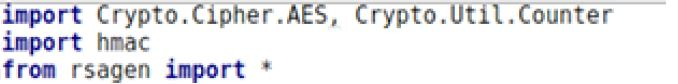
\includegraphics[width=8cm, height=1.5cm]{./images/Interfaz/07.jpg}
			\caption{Seleccionar Archivo}
			\label{fig:6-4-7} 
			\end{figure} 


\begin{itemize}
	\item  La biblioteca \textbf{Crypto.Cipher.AES} tiene implementado el algoritmo AES en todas sus versiones y lo utilizaremos para cifrar.
	\item  La biblioteca \textbf{hmac} contiene la implementación de las funciones Hash que parael desarrollo de este protocolo criptográfico se utilizó \textbf{SHA256}.
	\item La biblioteca \textbf{rsagen}, en ésta implementamos el algoritmo de RSA para la generación de llaves.

\end{itemize}



En ésta parte de la codificación, se tiene la implementación de la función \textit{subir archivos}, donde lo primero que hacemos es abrir las llaves del servidor y crear una conexión con ayuda de sockets entre nuestro cliente y el servidor.
			\begin{figure}[H]
			\centering
			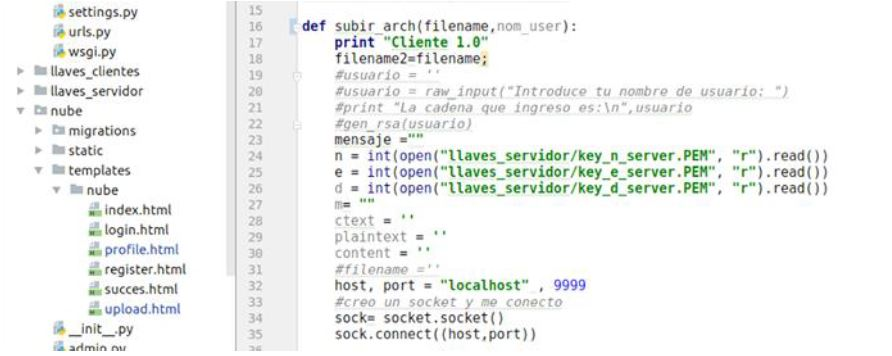
\includegraphics[width=17cm, height=7cm]{./images/Interfaz/08.jpg}
			\caption{Conexión con Sockets}
			\label{fig:6-4-8} 
			\end{figure}



Una vez creada la conexión  entre cliente - servidor, se obtiene el archivo que se va a subir, esto gracias a que cuando se manda a llamar la función, ésta pasa por parámetros el nombre del archivo y del usuario. Con esto se logra abrir el archivo y se le aplica una función hash de \textit{SHA256 (h(m))} y se opera con la llave pública del servidor \textit{(e)}, a esto se le llama \textit{factor de ocultamiento (x)}, con este factor se puede llevar a cabo una firma a ciegas por parte de nuestro servidor, éste factor se le envía al servidor por medio de  sockets.

			\begin{figure}[H]
			\centering
			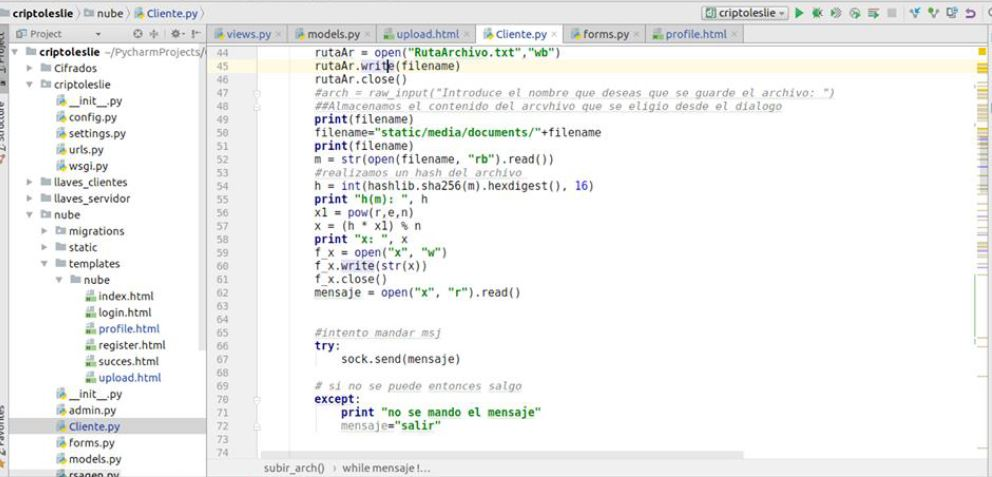
\includegraphics[width=17cm, height=8cm]{./images/Interfaz/09.jpg}
			\caption{Factor de Ocultamiento}
			\label{fig:6-4-9} 
			\end{figure}

Una vez realizada la firma a ciegas \textit{(y)} la envía al cliente por medio de sockets, el cuál procede a calcular la llave \textit{z} (que sirve para cifrar los archivos). Y se crea un archivo con dicha llave, ya que esta llave es demasiado grande para que funcione en AES, es por ello que se debe de sacar un hash con \textit{SHA256} para que quede del tamaño permitido por \textit{AES (128 bits)} y de igual manera creamos un archivo con la llave.

			\begin{figure}[H]
			\centering
			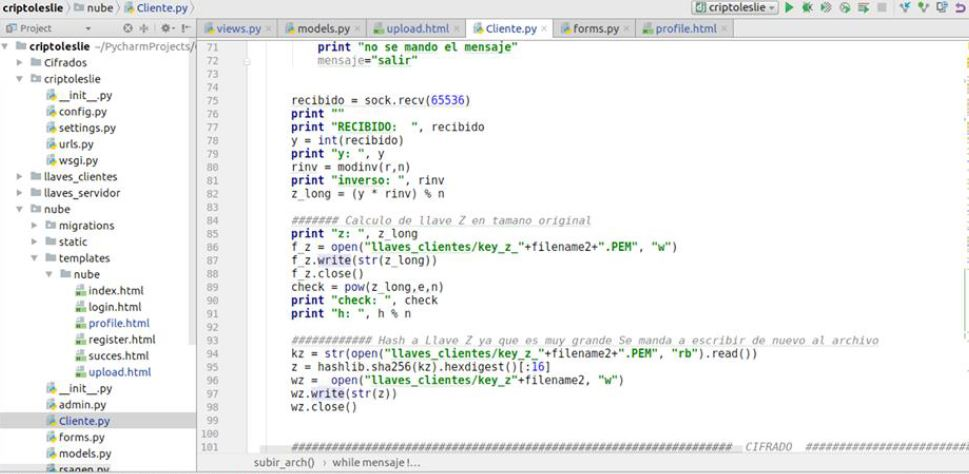
\includegraphics[width=17cm, height=9cm]{./images/Interfaz/10.jpg}
			\caption{Cálculo de Llave Z}
			\label{fig:6-4-10} 
			\end{figure}

Para cifrar el archivo se guarda el contenido de la llave \textit{z} y es utilizada para generar un vector de inicialización usando una función \textit{SHA256}, dicho vector se almacena en un archivo para que pueda ser utilizado posteriormente a la hora de descifrar el archivo, posteriormente se cifra el archivo con ayuda de las funciones definidas en las bibliotecas criptográficas que se mencionan anteriormente, y se le indica el tamaño de la llave de \textit{128 bits}, con un modo de operación \textit{CTR} y con la función \textit{encrypt()} se cifra el archivo, éste archivo se almacena en una carpeta y se le pone el nombre original pero agregandole una  extensión \textit{.aes}

			\begin{figure}[H]
			\centering
			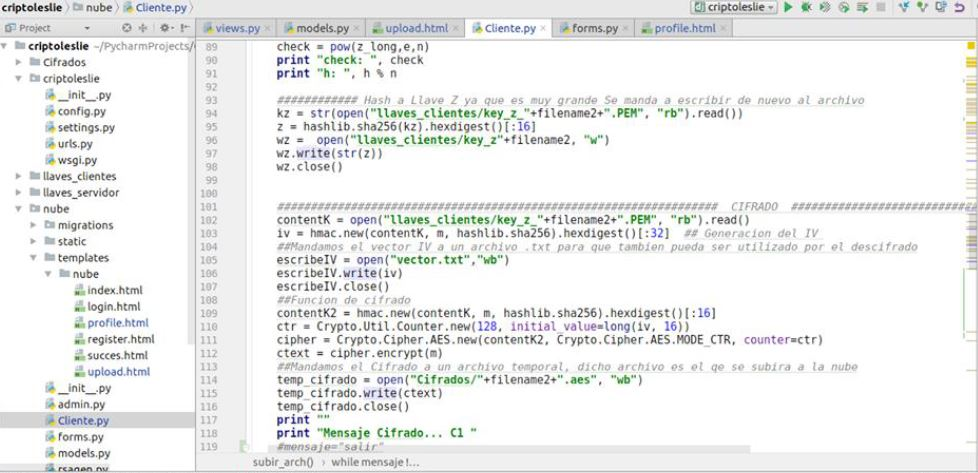
\includegraphics[width=17cm, height=9cm]{./images/Interfaz/11.jpg}
			\caption{Cifrado de Archivo}
			\label{fig:6-4-10} 
			\end{figure}



